\documentclass[10pt,a4paper]{article}
\usepackage[utf8]{inputenc}
\usepackage[T1]{fontenc}
\usepackage{amsmath}
\usepackage{amsfonts}
\usepackage{amssymb}
\usepackage{graphicx}
\usepackage{tikz}
\usepackage{float}

\usetikzlibrary{fit,positioning}

\author{Gabriel Wallin}
\title{Some notes on state-space LBM}

\begin{document}
\maketitle


\section{Graphical representation of the model}
\begin{figure}[H]
	\centering
	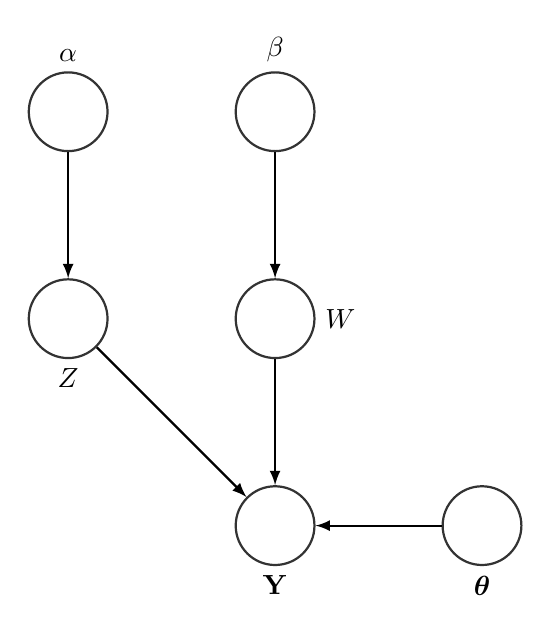
\begin{tikzpicture}
		\tikzstyle{main}=[circle, minimum size = 10mm, thick, draw =black!80, node distance = 16mm]
		\tikzstyle{connect}=[-latex, thick]
		%\tikzstyle{box}=[rectangle, draw=black!100]
		\node[main, fill = white!100] (alpha) [label=above:$\alpha$] { };
		\node[main] (Z) [below=of alpha,label=below:$Z$] { };
		
		\node[main] (beta) [right=of alpha, label=above:$\beta$] { };
		\node[main] (W) [below=of beta,label=right:$W$] { };
		
		\node[main] (Y) [below=of W, label = below:$\mathbf{Y}$] { };
		\node[main] (theta) [right=of Y, label = below:$\boldsymbol{\theta}$] { };
		
		\path (Z) edge [connect] (Y);
		\path (W) edge [connect] (Y);
		
		\path (theta) edge [connect] (Y);
		
		\path (alpha) edge [connect] (Z);
		\path (beta) edge [connect] (W);
		
		
		%\node[rectangle, inner sep=0mm, fit= (z) (w),label=below right:N, xshift=13mm] {};
		%\node[rectangle, inner sep=4.4mm,draw=black!100, fit= (z) (w)] {};
		%\node[rectangle, inner sep=4.6mm, fit= (z) (w),label=below right:M, xshift=12.5mm] {};
		%\node[rectangle, inner sep=9mm, draw=black!100, fit = (theta) (z) (w)] {};
	\end{tikzpicture}
\end{figure}	

$\mathbf{Y} = (Y_t^I, Y_t^R)^\top$ and $\boldsymbol{\theta} = (\theta_t^S, \theta_t^I, \theta_t^R)^\top$, where $Y_t^I$ is the proportion of infected at time point $t$, $Y_t^R$ is the proportion of removed at time point $t$, and $\theta_t^S$, $\theta_t^I$ and $\theta_t^R$ is the probability of a person being susceptible, infected and removed, respectively, at time point $t$.

$\mathbf{Y}$ is the data matrix where each element $\mathbf{y}_{ij}$ is a multivariate time series (bivariate for this particular case): $\mathbf{y}_{ij} = (y_{ij}^I(t), y_{ij}^R(t))$.

The density of of $\mathbf{y}_{ij}$:
$$
f(\mathbf{y}; \boldsymbol{\theta}) = \sum_{(z, w) \in \mathcal{Z}, \mathcal{W}} \prod_{i, g} \alpha^{z_{ig}} \prod_{j, l} \beta^{w_{jl}} \prod_{i, j, g, l} \varphi(\mathbf{y}_{ij}; \theta_{gl})^{z_{ig} w_{jl}}
$$

From the state-space model formulation, we know that 
\begin{align*}
	y_{ij}^I \sim \text{Beta}(\lambda^I \theta_t^I, \lambda^I(1 - \theta_t^I)) \\
	y_{ij}^R \sim \text{Beta}(\lambda^R \theta_t^R, \lambda^R(1 - \theta_t^R)
\end{align*}

So should we model $\varphi(\cdot)$ as a bivariate beta distribution?

Further we know from the eSIR model that 
$$
\boldsymbol{\theta}_t | \boldsymbol{\theta}_{t-1}, \boldsymbol{\tau} \sim \text{Dirichlet}(\kappa f((\boldsymbol{\theta}_{t-1}, \rho, \pi))),
$$
where $\kappa$ scales the variance of the Dirichlet distribution, and the function $f(\cdot)$ is a 3-dimensional vector that sets the mean of the Dirichlet distribution.

There is a paper ("Estimation and selection for the latent block model on categorical data" by Keribin et al.) that implements the LBM for multinomial data that in the estimation of the model sets prior distributions for the mixing proportions as well as the parameter that governs the $Y$ distribution. This would in a sense be similar to our case, since the eSIR model imposes a Dirichlet prior on the $\boldsymbol{\theta}$ parameter. If we would further impose Dirichlet priors on the mixing proportions, would we be able to do something similar as in Keribin et al.?

Regarding the function $f$, it is the solution to the SIR differential equations:
$$
\frac{\theta_t^S}{dt} = -\rho\theta_t^S\theta_t^I, \quad \frac{\theta_t^I}{dt} = \rho\theta_t^S\theta_t^I - \pi \theta_t^I, \quad \frac{\theta_t^R}{dt} = \pi \theta_t^I,
$$
Since there are no explicit solutions available to such a system of ordinary differential equating, the so-called fourth-order Runge-Kutta approximation is implemented.

The total set of model parameters equals $\boldsymbol{\tau} = (\alpha, \beta, \rho, \pi, \mathbf{\theta}, \lambda, \kappa)^\top$. Should be possible to estimate using MCMC?

\end{document}